%TODO IHE profiles explicar

\chapter{International Practices and Conventions}\label{chap:standards}

\section*{}

In this chapter, the objective is to present the main Health International Standards for interoperability, helping us to understand which options there are to allow the systems to properly share, interpret and store data. In addition, we analyse two EHR implementations case studies, from Canada and England.


%%========================================
%% Health internacional standards
%%========================================
\section{Health International Standards}

The pursuit of interoperability is not possible without the clearly definition of common languages and communication channels. These common languages are called standards and are usually created and managed by independent organizations.

\subsection{Health Level Seven International}

Health Level Seven International (HL7) is one of several accredited organizations of American National Standards Institute (ANSI), operating in the healthcare area. HL7 provides a set of standards towards interoperability, aiming to facilitate knowledge transfer among several stakeholders: healthcare providers, government agencies, patients and so forth~\citep{Seven}.


\subsubsection{HL7 Messaging Standard}

One of the most used standards is the messaging one. The HL7 Messaging Standard appeared several years ago and had been evolving along the last two decades. Several institutions adopted and implemented it all over the world, most of the times investing lots of time and money to achieve it. Dave Shaver stated some interesting numbers~\citep{Shaver2010} about the utilization of the different standard versions, which are resumed in Figure~\ref{fig:hl7-version-comparasion}. By observing the Figure~\ref{fig:hl7-version-comparasion}, we can easily conclude that ``the vast majority of HL7 messaging is done using messages that approximate HL7 2.3 or HL7 2.3.1'' unlike the newer ones (2.5 or greater and 3.0) that represent a ``very small portion of real-world interfaces''~\citep{Shaver2010}.

\begin{figure}[t]
\centering
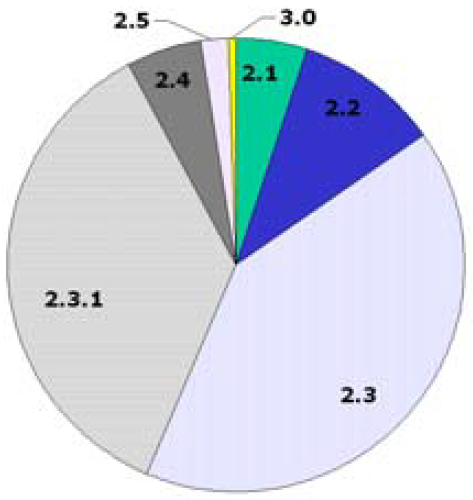
\includegraphics[width=0.35\textwidth]{HL7-versions-comparasion}
\caption[Approximate real-world usage of HL7 messaging standards]{Approximate real-world usage of HL7 messaging standards~\citep{Shaver2010}}
\label{fig:hl7-version-comparasion}
\end{figure}


\subsubsection{HL7 Messaging Standard Version 2} \label{sec:hl7-v2}

The HL7 v2 is a standard created several years ago. Nevertheless, it had evolving into some new versions. Currently, HL7 v2 is at version 2.7. However, as it was designed as backwards compatible, the version is not so relevant. In fact, what is often more important is how the system which is sending the message is populating the fields and segments the standard defines. 

The HL7 v2 stands as a simple protocol for exchanging clinical data and it stands as the most widely used healthcare information standard~\citep{Eichelberg2005}. Certainly, one reason for that is that the referred messages are plain text, with several fields split by the vertical slash character `|' as it is possible to observe in Figure~\ref{fig:hl7v2-msg}.

\addtocounter{footnote}{1}
\begin{figure}[t]
\centering
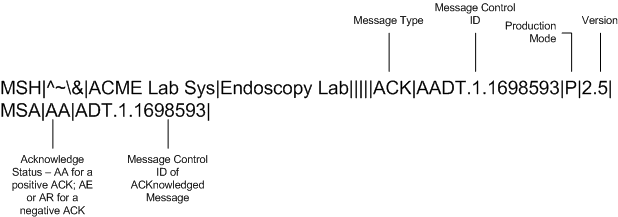
\includegraphics[width=0.9\textwidth]{HL7V2Message}
\caption[Example of an HL7 v2 acknowledgement message]{Example of an HL7 v2 acknowledgement message$^{\decimal{footnote}}$}
\label{fig:hl7v2-msg}
\end{figure}
\footnotetext[\value{footnote}]{Source: \url{http://www.interfaceware.com/images/ACKMessageAnatomy.png}}

However, some authors advocate that ``the messages lack a formal underlying reference model, and feature considerable optionality in addition to permitting user-defined elements''. In fact, that excessive flexibility obliges to establish a prior agreement structure and interpretation that might be called ``negotiated interoperability''~\citep{Atalag2010}. Obviously, this vagueness ``provides great flexibility but necessitates detailed bilateral agreements among the healthcare systems to achieve interoperability'' as state Eichelberg \textit{et al}~\citep{Eichelberg2005}.

In this context, it is important to clearly identify the main advantages of using HL7 v2, which we point out next~\citep{Atalag2010}:
\begin{itemize}
\item richly expressive data types;
\item support for arbitrary structured objects;
\item easy to adopt and use with low cost.
\end{itemize}

As expected, there are some arguments against also, which are:
\begin{itemize}
\item excessive flexibility and optionally in message interpretation implies a  ``negotiated interoperability'';
\item lack of privacy and consent guarantees;
\item growing tendency to abandon v2 in favour of v3. 
\end{itemize}

To conclude, despite of being an exceeded standard it is still very relevant, being used world wide. 

\subsubsection{HL7 Messaging Standard Version 3}

The HL7 v3 appeared as a natural evolution of HL7 v2, trying to solve some problems that the previous version had. Its first version was launched in 2005. Despite of being just a new release, this update means significant standard modifications as the main objective was to ``establish semantic interoperability in loosely coupled systems''~\citep{Atalag2010}. In this sense, at the core of this standard just appeared the Reference Information Model (RIM).

The RIM is an object model created as part of the Version 3 methodology, serving as a context provider to the multiple healthcare concepts. For instance, a WBC (white blood count) may refer to an order (intent) or a result (observation). In that case, the RIM structures ``implement the context by binding the coded vocabulary term from the ontology to a specific place in the model''~\citep{Shafarman2004}.

With HL7 v3, the messages are no longer plain text but XML files (as we can see in Figure~\ref{fig:hl7v3example}) which turns the message more human-readable but also more structured and rigid.

\begin{figure}[t]
\centering
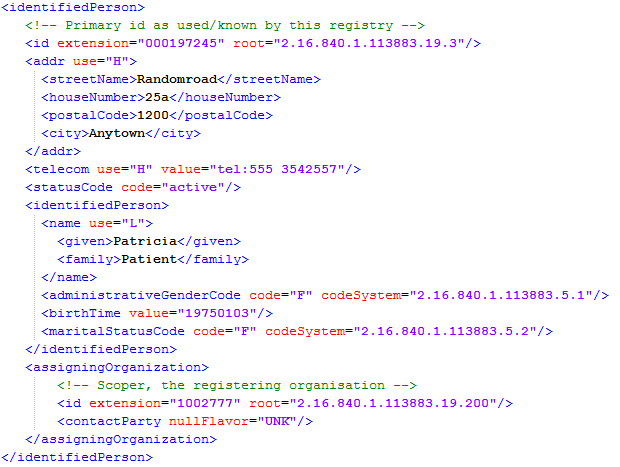
\includegraphics[width=0.86\textwidth]{hl7v3example}
\caption[Example of an HL7 v3 message]{Example of an HL7 v3 message~\citep{Spronk2007}}
\label{fig:hl7v3example}
\end{figure}

There are some advantages that should be credited to this Version 3, which are important to summarize~\citep{Atalag2010,Shaver2010}:
\begin{itemize}
\item rich in clinical semantics;
\item address many of the practical difficulties such as incomplete information, uncertainty, duplicate records and so forth;
\item dynamic model no more complex than v2;
\item ``less expensive to build and maintain mid-to-long term interfaces'';
\item ``more of a `true standard' and less `framework for negotiation''';
\item the long journey of maturing and reflecting about the standard.
\end{itemize}

Notwithstanding of the several advantages, there are some drawbacks that can be identified~\citep{Atalag2010,Shaver2010}:
\begin{itemize}
\item not clear where the return of investment is since it does not offers substantial advantages over v2 for some areas (simple alerting, drug interaction checking, recall systems, best practice guidelines, clinical pathways, and so forth);
\item message structures complex and difficult to understand;
\item ``inconsistencies between an Information Model (objects document things) interpretation and a Reference Ontology (objects are things) interpretation'';
\item not suitable as a model for storage EHR information and does not specify and EHR Architecture neither;
\item unclear how is it possible to query a v3 messages repository;
\item absence of compatibility with HL7 v2; 
\item expensive and slow adoption.
\end{itemize}

In an interesting research by Gartner in 2006, Rishel predicted that ``the HL7 V3 messages will fail to achieve critical mass, being replaced by ever-more-elaborate use of V2, a series of dialects of V3 chosen by individual countries and large enterprises, or the work of other standards organizations that may achieve less semantic interoperability while being easier to implement''~\citep{Rishel2006}.

To complete, the HL7 v3 seems the natural evolution for the applications using the previous versions. Although, that migration will take many years and it might not be so pacific as would be desirable.


\subsubsection{Clinical Document Architecture (CDA)} \label{sec:hl7-cda}
Clinical Document Architecture (CDA) is an ANSI-certified standard from HL7 organization. The first version (Release 1.0) was released in November, 2000 and the second (Release 2.0) was published with the HL7 2005 Normative Edition.~\citep{Seven} CDA defines the semantic and structure of clinical documents aiming to allow its exchanging. The CDA documents are actually XML documents. That concept is derived from the fact that these documents ``derive their meaning from the HL7 Reference Information Model (RIM) and use the HL7 Version 3 Data Types which are part of the HL7 RIM''~\citep{Atalag2010}.

The CDA document is constituted by two parts, an header and a body. The header is used to unambiguously state the semantics of each entry in the document. The body ``contains the clinical document content and can be either an unstructured text, or comprised of nested containers''~\citep{Eichelberg2005}.

It is important to distinguish the two versions of this standard, since there are many applications that still use the first version. The main characteristic of CDA standard is the documents classification into three different levels, although the interpretation of them is differentiated between the two versions.

The CDA Release One considers two levels~\citep{Seven,Eichelberg2005}:
\begin{itemize}
\item Level One --- basically it has a standardized header and additional information on the rest of the document;
\item Level Two --- allows to define and constraint both the structure and the content of the document, favouring the interoperability between systems since the receiver knows what to interpret;
\end{itemize}

The approximation of CDA Release Two is a little different. In fact, it provides an incremental approach, allowing and encouraging the documents to evolve and becoming more structured. One of the major additions is that the CDA body ``uses RIM structures and controlled vocabulary to permit a much higher level of semantic interoperability''~\citep{Seven}. Atalag \textit{et al} advocate that it is a ``stable and flexible standard for developing communications with coded information'' as well as ``provides a pathway from narrative free text documents through incrementally coded data to fully coded and semantically interoperable clinical data''~\citep{Atalag2010}.



\subsection{The openEHR} \label{sec:openehr}

The openEHR standard is a standard owned by the openEHR Foundation, created in 2002. The Foundation is a non-for-profit organization with the founding partners being University College London and Ocean Informatics, an Australian company. The main objective is to research and develop interoperable electronic health records related topics, aiming to improve the care quality to patients~\citep{Leslie2007}.

Unlike other standards, openEHR develops specifications for implementing full EHR systems, pronouncing more in persistence as opposed to messaging. openEHR states that, in order to achieve lifelong, patient centred, secure and shareable EHR, the way cannot be the aggregation of messages~\citep{Beale2002}.

In order to provide an high level of interoperability, openEHR suggests the engaging of standardized clinical content models (called Archetypes), a stable reference model and semantically rich terminologies~\citep{Atalag2010}. More in detail, Bale advocated a two-level methodology to model the EHR structure. In the first level, the existence of a generic reference model, specific to the healthcare domain but sufficiently general to be stable over the time (e.g. role, act, entity and so forth). In the second level, there were concepts mapped as archetypes, such as blood pressure, laboratory results and so on. The archetypes apply ``constraint rules  that specialize the generic data structures that can be implemented using the reference model''~\citep{Beale2002}.

Beyond the reference information model, the openEHR framework includes other resources that help the implementation following this standard, such as the ADL (Archetype Definition Language) language for expressing archetypes, an archetype library and a collection of open source implementations. As an example (Figure~\ref{fig:openehr-adl}), we can restrict a generic Observation class to, for example, a Blood Pressure archetype.

\begin{figure}[t]
\centering
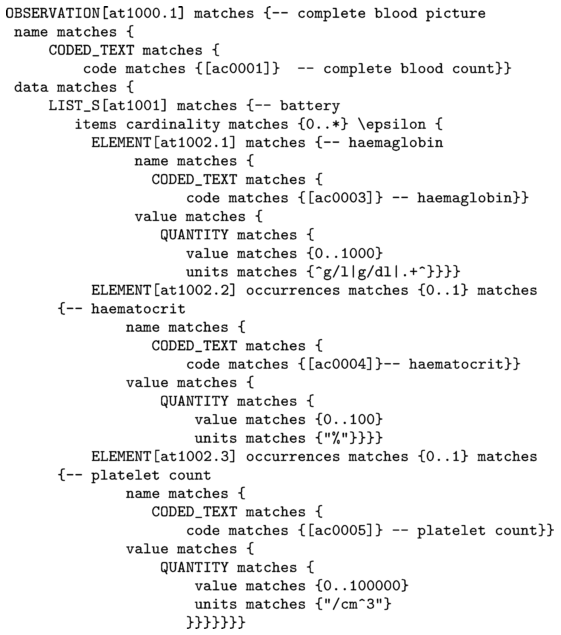
\includegraphics[width=0.7\textwidth]{openehr-adl}
\caption[The ADL definition of Complete Blood Count archetype]{The ADL definition of Complete Blood Count archetype ~\citep{Eichelberg2005}}
\label{fig:openehr-adl}
\end{figure}



\subsubsection{Advantages and Disadvantages}

There are some interesting characteristics about openEHR that might be useful to underline~\citep{Atalag2010}:
\begin{itemize}
\item intuitive and understandable model for clinicians;
\item approach based on recording and querying observations;
\item extracts can be sent with HL7 v2 (see~\ref{sec:hl7-v2});
\item likely stable reference model	over the time;
\item possibility to convert archetypes into CDA documents (see~\ref{sec:hl7-cda}).
\end{itemize}

On the other hand, Atalag \textit{et al} identified some arguments against either~\citep{Atalag2010}:
\begin{itemize}
\item ``lacks semantic rigour and does not contain a logically sound ontology'';
\item works well with simple scenarios, but does not easily handle complexity;
\item no experiences with medium to large-scale systems;
\item weak governance of the openEHR Foundation.
\end{itemize}

To conclude, the interest with this standard is spreading worldwide. There is an increasing number of full or partial implementations of the openEHR specifications in several countries, like United Kingdom, Sweden, Australia, Denmark, The Netherlands, Singapore, USA, Japan, Brazil, Scotland or Turkey. However, there is not a really large-scale systems in neither of these countries and the use of the standard consists of using some of its concepts~\citep{Atalag2010}. In another interesting article, Marta Silva and José Carvalho state that the ``openEHR standard has original and sound fundamental
concepts that definitely will influence future generations of health information systems'' as long as note that ``some openEHR core beliefs are highly debatable''. Also, they raise some questions about the applicability of semantic interoperability ``when the industry all over the world is struggling in exchanging basic unstructured demographic and clinical data through the complex network of health providers''.~\citep{SilvaMarta;Carvalho2011}




\subsection{Integrating Healthcare Enterprise} \label{sec:ihe}

The Integrating Healthcare Enterprise (IHE)~\citep{IHE_PROFILES} is an initiative from healthcare professionals and industry that work to improve the way health care systems share information electronically. The group was formed in 1998 as a cooperative venture by the Healthcare Information and Management Systems Society (HIMSS) and the Radiologic Society of North America (RSNA) with the goal to promote interoperability among imaging and health care information systems. 

IHE is an international organization that focuses on the development of open and global IHE Integration Profiles and on the regional deployment of interoperable IT systems. IHE encourages the use of established interoperability standards such as HL7 and DICOM.

\subsubsection{IHE Profiles} \label{sec:ihe_profiles}
IHE strives to solve specific integration problems faced by its membership in the real world through Integration Profiles. These profiles define the systems involved (i.e., actors), the specific standards used, and the details needed to implement the solution. Each profile offers developers clear communication standards that have been reviewed and tested by industry partners. A group of systems that implement the same Integration Profile address the need/scenario in a mutually compatible way. Some examples of IHE Profiles are:
\begin{itemize}
\item Cross-enterprise Document Media Interchange (XDA) -- transfers documents and meta-data using CDs, USB memory or email attachments;
\item Cross-enterprise Document Reliable Interchange (XDR) -- exchange of health documents between health enterprises using a web-based, point-to-point push network communication;
\item Patient Identifier Cross Referencing (PIX) -- cross-referencing multiple local patient IDs between hospitals, sites, health information exchange networks, etc.
\end{itemize}

\subsection{Digital Imaging and Communications in Medicine} \label{sec:dicom}

DICOM (Digital Imaging and Communications in Medicine) is an worldwide used standard for medical image communication. The standard provides data structures and services allowing the exchange of medical images and related information. In the actual structure, the standard is available since 1993, despite the creation remounts to 1983.

Unlike most of other EHR standards, the DICOM uses a binary encoding. Pianykh has an interesting point of view, saying that ``contrary to popular belief, DICOM is not just an image or file format'' but ``an all-encompassing data transfer, storage, and display protocol built and designed to cover all functional aspects of digital medical imaging''~\citep{Pianykh2008}.

Other authors stated that ``it has become a leading standard used by all major vendors of diagnostic medical equipment'', predicting also that ``DICOM will soon be used in every medical branch that utilizes imaging, for example: cardiology, mammography, radiology, surgery, endoscopy, dentistry, pathology, etc''~\citep{Mustra2008}.


\subsection{Terminology and Ontology Standards}

The need of data sharing between different healthcare institutions leverage the creation of multiple standards, attempting to allow, not only the data sharing, but also the easy interpretation of the message's content. in fact, this kind of internationally endorsed classifications facilitate the storage, retrieval analysis and interpretation of data. In this sense, in the next subsections we will present some terminologies that were created with the aim of making the systems understand each other.

\subsubsection{Systematized Nomenclature of Medicine - Clinical Terms} \label{sec:snomed}

SNOMED CT (Systematized Nomenclature of Medicine - Clinical Terms) was created in 2006 by the International Health Terminology Standards Development Organisation (IHTSDO). This standard aims to provide a unique and embracing system with clinical terms. The objective is to have a repository, managed and updated centrally, available to all systems which adopted it and that can be used either to clinical purposes as to research projects.~\citep{ACSS/MS2009a}

Citing the official site, the SNOMED CT ``provides the core general terminology for the electronic health record (EHR) and contains more than 311,000 active concepts with unique meanings and formal logic-based definitions organized into hierarchies'' and ``can be used to represent clinically relevant information consistently, reliably and comprehensively as an integral part of producing electronic health records''~\citep{IHTSDO}.


\subsubsection{International Classification of Diseases} \label{sec:icd}

The International Classification of Diseases (ICD)~\citep{WHO} is ``the international standard diagnostic classification for all general epidemiological, many health management purposes and clinical use''. This standard is owned by the World Health Organization (WHO) and dates from 1850, being developed and reviewed every ten years. Although, every year new updated are release to the versions in use. The ICD provides an huge variety of codes to classify diseases, body signals, symptoms, abnormal aspects, complaints, social circumstances and external causes of injury or illness, beyond to having an additional classification used to classification of transplants and newborns and so forth. 

ICD is a classification, and a essential one, as it define the universe of entities to be studied, and highlight the relevant aspects of the information that has been collected. Also, it allows their comparison in several contexts: within and between populations over time and the compilation of internationally consistent data.

%TODO Logical Observations Identifiers Names and Codes (LOINC)

%\subsection{Overview}

%TODO meter tabela com comparação de standards como tem o lucas ribeiro






%%========================================
%% Internacional case studies
%%========================================

\section{International Case Studies}

Several Electronic Health Record projects were initiated in multiple countries. The study of same of those might be fundamental in order to understand what can we learn with them. By doing that, it will help us to extend our horizons, retain the bad experiences and better evaluate some options that we might have to take.

In the next subsections, we will provide an overview by two EHR initiatives: the Canada Health Infoway and the National Health Service (from England).

\subsection{Canada Health Infoway}

Canada Health Infoway is an non-for-profit organization founded by Canada's First Ministers in 2001. It was specifically created to accelerate the process of development of Electronic Heath Record systems, promoting the adoption of standards that guide to communication facilitation between different healthcare organizations. 

In order to guide the development of the systems in each different province, Infoway provided a national framework called EHR Blueprint. The EHR Blueprint is a set of principles, guides and components. It states ``a comprehensive description of the components necessary for the interoperable EHR and describes, in broad terms, how the components are envisioned to work together''~\citep{April2006}.

\subsubsection{Sharing EHR Information} \label{sec:share-ehri}
In the process of building an EHR, there are several methods to allow sharing EHR information along several services, consumers and providers. EHRS Blueprint advocates that the best method (at least for their reality) is the creation of a shared reference information source that is populated by several health-care organizations around Canada. This reference is populated with clinical relevant data and is maintained externally from ever health-care organization (or Points of Service, as designated in EHRS Blueprint). The Points of Service (PoS) are able to reference or pull data from the shared repository.

The `EHR Infostructure' is based on achieving full integration and interoperability between the EHR Solution and each PoS. In order to do so, EHRS Blueprint has a Health Information Access Layer that provides the interface which all the PoS communicate with. However, since EHRS Blueprint defines an unique interface for all PoS, most of these systems needed to adapt themselves to respect the standards and be able to stay connected to the system. 

This shared reference presupposes the existence of peers along each different Canada's jurisdiction. These peers represent several copies of the EHRi in terms of structure, but dealing only with the local PoS. As the infrastructure is the same, the process of retrieving information from other peers, when needed, is relatively simple.


\subsubsection{Architectural principles}

The EHRS Blueprint states~\citep{April2006} some architectural principles which guided the EHRs implementation. However, we will just point out the ones that might be more relevant and interesting at this point.

The fact of the EHR Infostructure information being stored as copy of the original one is a key characteristic, as it preserves independence between the EHRi and the PoS.

Another relevant principle is the controlled environment built around the system, defining one common interface and transforming EHRi into a black-box in which PoS can retrieve but also update clinical information for a specific patient.

The EHRS Blueprint was built following an Services Oriented Architecture, making the architecture more flexible and the components reusable. 

Another interesting fact is that there is no single `home' for the patient's electronic health record. Actually, each jurisdiction's EHRi holds and owns the data generated in health services from that jurisdiction.

\subsubsection{Key elements}

The EHR Blueprint has multiple components with certain characteristics. Although some of those had been already referred, it is useful to take a deeper look at them and point out some others also. Thus, the key elements are~\citep{April2006}:

\begin{figure}[t]
\centering
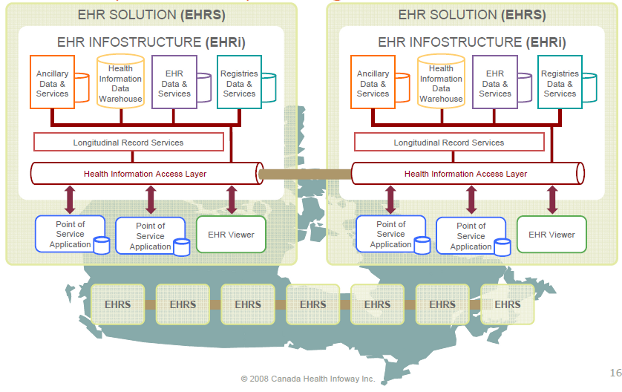
\includegraphics[width=1.0\textwidth]{blueprint-architecture}
\caption[EHRS Blueprint Architecture overview]%
			{EHRS Blueprint Architecture overview~\citep{Infoway}}
\end{figure}

\begin{itemize}
\item \textbf{Point of Service Applications (PoS)} --- these are software applications or information systems that provide clinical information to the EHR system, working as gateway for gathering critical patient data, absolutely fundamental to the system's purposes. It is important to notice that these systems are responsible for most collection of the patient's EHR data. Here, we refer to applications as an information system in hospital emergency department as well as an local pharmacy system and further so;

\item \textbf{EHR Data Repositories} --- sometimes, there is relevant clinical information that is no available in the PoS applications despite of being very relevant in a clinical decision making context. Instead, it is usually available through other systems. In this sense, the PoS applications are also responsible for pushing the data into these EHR Data Repositories -- that become responsible for storing it and keeping it available to the users that might need that. Four logical clinical domain repositories are identified by EHRS Blueprint: Shared Health Record, Drug Information, Diagnostic Imaging and Laboratory;

\item \textbf{Registry Services} --- there are the information linkers. There Registry Services provides the identification of patients, matching them with the required clinical data. In order to guarantee the match of required and retrieved information, these services offer: Client Registry, Provider Registry, Location Registry and Terminology Registry;

\item \textbf{Longitudinal Record Services (LRS)} --- as we saw in Subsection~\ref{sec:share-ehri}, the EHRS Blueprint is based on distributed data repositories. Thus, when it is needed to retrieve and show the information to the user (for instance, a physician), all the data must be gathered as if it was stored in the same place. These Longitudinal Record Services execute that task, bringing together data from different registries and sources, normalizing it for common understanding;

\item \textbf{Health Information Access Layer (HIAL)} --- it provides a single standardized way of sharing and retrieving data from EHRi. The fact of being unique and the single entry point obligates the PoS applications to adapt themselves to the interface but also to the information standards also. 
\end{itemize}


\subsection{England National Health Service}

The National Health Service (NHS) Connecting for Health is part of the UK Department of Health. This organization was created on 1 April 2005 as the replacement for an older one (NHS Information Authority). It has the responsibility of managing and implementing the NHS National Programme for IT (NPfIT). The NPfIT was an initiative to upgrade the NHS to a centrally-mandated electronic health record  for patients, connecting hundreds of hospitals and thousands of healthcare professionals and providing them relevant patient data by secure and certified means.


\subsubsection{Architecture overview}

The NPfIT has born as the world's largest civil information technology project, committing £12.4 billion over 10 years in order to improve the quality of healthcare in England. As expected, such a big project could not be just a single standalone implementation. In fact, the NPfIT is made of eight separated systems, which are~\citep{Brennan2005}: 
\begin{itemize}
\item \textbf{One National Application Service Provider (NASP)} --- designed to support the `National Data Spine', which was destined to keep the patients' electronic data;
\item \textbf{A New National Network (N3)} --- a network connecting all the hospitals, applications and other healthcare providers, characterized by the need of being a really broadband one. It would be an essential infrastructure supporting and linking all the other services providers;
\item \textbf{One Electronic Appointment Booking (eB)} --- a service (now called `Choose and Book') that would give the possibility of the patients to choose the place, date and time for their appointments in a hospital or clinic;
\item \textbf{Five Local Service Provider (LSP)} --- five physically distributed providers, hosting the NHS Care Records Service (NHS-CRS) at a local level, covering all England's territory.
\end{itemize}

\begin{figure}[t]
\centering
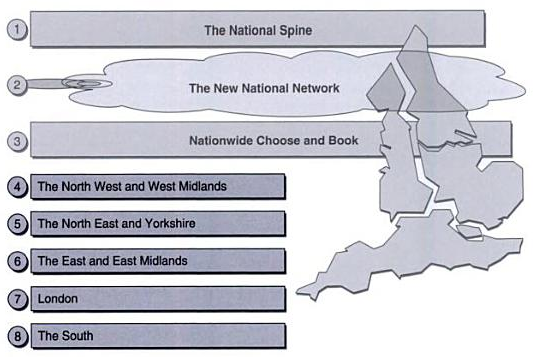
\includegraphics[width=0.7\textwidth]{npfit-architecture}
\caption[The England's National Programme for IT]{The England's National Programme for IT~\citep{Brennan2005}}
\label{fig:npfit-architecture}
\end{figure}

The Figure~\ref{fig:npfit-architecture} briefly describes the kind of interaction between the different components of the system. It is important to notice that, in order to implement the five local clusters, five providers were contracted and made responsible for delivering the local services. The idea was that, in one hand, the providers would be challenged to compete between each other, speeding up the process of implementation. On the other hand, the risk would be lower since there was different suppliers implementing similar systems in parallel. CSC Alliance, BT Health London, Accenture and The Fujitsu Alliance were the contracted LSP's for the main body of the programme.


\subsubsection{NHS Interoperability Toolkit (ITK)}
The NHS Interoperability Toolkit is a set of standards, frameworks and implementation guides to support and favour the interoperability between local systems and across them. The NHS ITK aims to support flexibility and local innovation and also removing barriers to entry. It also wants to be an enabler of evolution and reusing of solutions that already proved to be valuable, connecting all the peers by standardization in order to ensure that there are no silos being created.

One of the key concepts of ITK is the use of a maturity-based approach, allowing the organizations to evolve through small steps, particularly for CDA documents. The step-by-step maturity model allows the organization to incrementally progress from sharing binary data to sharing fully-coded CDA documents.

\begin{figure}[t]
\centering
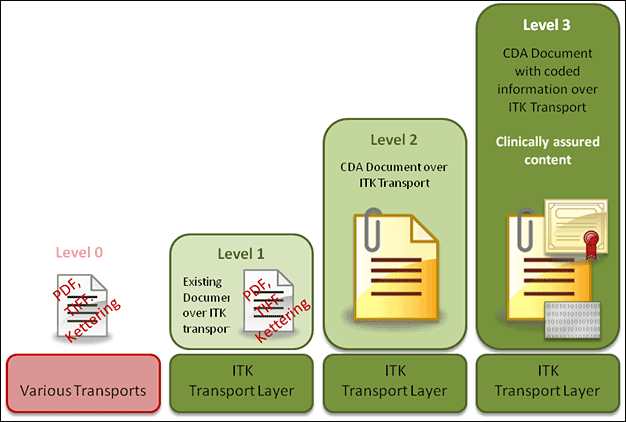
\includegraphics[width=0.8\textwidth]{itk-maturitymodel}
\caption[The NHS ITK Maturity Model]{The NHS ITK Maturity Model~\citep{Health2012}}
\label{fig:npfit-itk}
\end{figure}

As it is possible to observe in Figure~\ref{fig:npfit-itk}, there are four possible levels in the model. The lowest one -- Level 0 -- is applied to any organization, when even the sharing itself is made out of the ITK Transport Layer. When one organization becomes to use the ITK Transport Layer it reaches the Level 1. Then, the Level 3 is assigned when an organization is able to share CDA documents. Finally, when the data is passed through CDA documents one organization has reached the highest level -- Level 4. In Section~\ref{sec:hl7-cda} we explain the CDA standard more in detail.


\subsubsection{NHS Care Records}
The NHS Care Records is one of the NPfIT's components. This component is what we usually call an Electronic Health Record system, aiming to provide personal clinical information to the healthcare providers, increasing the quality and efficiency of the treatments.

The NHS Care Records considers two different types of records:
\begin{itemize}
\item \textbf{Summary Care Records} --- records held nationally. A Summary Care Record -- usually called Patient Summary -- stores essential information about a person, available in emergency situations, informing the health professionals about what medicines are one taking, the allergies that might suffer from or any known bad reactions to other medicines;
\item \textbf{Detailed Care Records} --- records held locally. The Detailed Care Record is a more comprehensive record which might store data from past exams and details, avoiding the necessity for repeating them, for example.
\end{itemize} 


\subsubsection{The fall and the failure}
The NPfIT started in October 2002 and since then it always been the target of some criticises. However, in April 2006, a set of 23 academics, wrote an open letter\footnote{Details: \url{http://editthis.info/nhs_it_info/The_Open_Letter_to_the_Health_Select_Committee}} raising several questions and concerns about the programme. A report by the King's Fund in 2007 also criticised the government's ``apparent reluctance to audit and evaluate the programme'', questioning their failure to develop a capable strategy~\citep{Wanless2007}.

The next years were very troubled as long as several reports raising doubts about the feasibility of the project were made public ~\citep{Powell2004,Coiera2007,Brennan2007,Clegg2007,Brennan2009}. One of those, by the Public Accounts Committee, stated in 2009 that the risks for the programme deployment were ``as serious as ever'', bringing up serious uncertainty about the capacity of the systems to meet expectations of clinical staff. \footnote{Details: \url{http://news.bbc.co.uk/2/hi/health/7850619.stm}} The over-and-over delays to deliver the fundamental services and the overrun of the programme's cost started to being unsupportable. In September 2011, the NPfIT has been dismantled following the conclusions of a new review by the Cabinet Office's Major Projects Authority (MPA)~\citep{OfHealth}.

